\section{Introduction to downfolding the many electron problem}

One of the most sought-after, yet often daunting, endeavors for physicists is to develop 
an intuitive understanding of physical phenomena involving intrinsically complicated materials 
using simplified models. These models are expected to capture the essence of the physics, and are formulated in terms 
of the most relevant physical degrees of freedom related to the observed phenomena. 
For example, at high temperature and low density when quantum effects are relatively insignificant, the ideal gas model 
successfully captures the statistical properties of $10^{23}$ H$_{2}$ molecules in a box, 
without any detailed knowledge of the fundamental constituent of H$_{2}$. This approach is valid when we are interested in 
phenomena at certain energy scale (or length scale), while the degrees of freedom at other length scales which are not 
dynamically excited simply renormalize the dynamics of the low energy degrees of freedom. 

This principle, the basis of the renormalization group~\cite{Wilson}, 
has also been widely employed in condensed matter physics. In the past few decades, several studies 
have been dedicated to describing complex systems (for example, the high $T_c$ cuprates and other transition metal oxides), those of 
primary interest here are strongly correlated systems. These are systems where the effects of Coulomb 
interactions are comparable to or more important than the kinetic energy and the picture of 
localized rather than itinerant electrons is more pertinent. This has motivated an approach beyond the 
traditional band theory approach, involving model Hamiltonians such as the Hubbard~\cite{Hubbard}, t-J~\cite{tJSpalek} 
and Heisenberg models, defined only in terms of the valence electrons. 
While these models have been extensively studied analytically and numerically, and have significantly 
enhanced our understanding of strongly correlated physics, their effectiveness 
for describing a real complex system of interest is often unclear. 
%In addition, efforts to obtain the optimal parameter values still remains very much an active area of research, often requiring experimental inputs. 
%This is compounded by the fact that all the parameters are not independent of each other and 
%the value of one heavily influences the value of the other. The presence of multiple competing energy scales of similar strength 
%is, in fact, the source of rich phase diagrams that 
%emerge under a variety of conditions - doping, pressure, 
%temperature, all heavily dependent on material-specific properties. 
This motivates the need to determine reliable low energy effective Hamiltonians that can capture all the necessary details, while 
remaining simple enough to be simulated accurately.  

\begin{figure}[htpb]
\centering
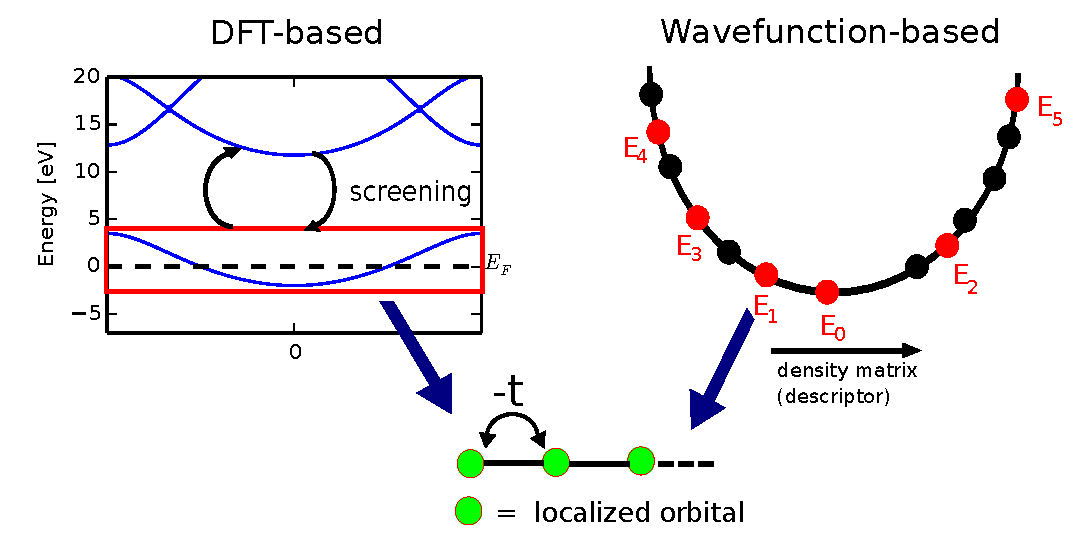
\includegraphics[width=1\linewidth]{./Figures/figure1.eps}
\caption{Schematics for downfolding a simple ab-initio system (here the hydrogen chain) 
in DFT based methods (left) and the wavefunction based AIDMD (right). Localized one particle functions 
are constructed in both methods and serve as the one body space for the model Hamiltonian. The DFT based methods 
use Kohn Sham orbitals and screening models to estimate the interactions. AIDMD uses a database of low energy 
all electron many-body wavefunctions ($\psi_i$). This "low energy basin" 
(shown abstractly in the space of descriptors) need not consist of exact eigenstates ($E_i$).}
\label{fig:lowenergybasin_schematic}
\end{figure}	


%In complex systems such as high $T_c$ cuprates, it is unclear to what extent can these models describe the reality \cite{Anderson2013}. 
%Since strongly correlated systems are  the macroscopic phenomena are strongly dependent on material-specific properties, motivating the need to determine the effective Hamiltonians that can capture all necessary details. 
%In strongly correlated systems, the macroscopic phenomena are strongly dependent on material-specific properties, motivating the need to determine the effective Hamiltonians that can capture all necessary details. 
%\HJC{Downfolding: How should we connect our intuitive understanding of coarse graining with condensed matter concepts}
%The reliable simulation of strongly correlated systems remains a major challenge in physics, chemistry, and materials science. 
%On the other hand are approximate model Hamiltonians (such as the Hubbard model) 
%which describe the low energy physics solely in terms of the valence electrons and 
%are crucial to our understanding of physical phenomena such 
%as antiferromagnetism and high temperature superconductivity. 
%However, transitioning from actual materials to an effective Hamiltonian on a lattice relies 
%on physical insight and/or fits to experimental data, and this notion is not always rigorously well justified.

The endeavor we pursue here is to develop a multi-scale approach in which the effective interactions between 
quasiparticles (such as dressed electrons) are determined after an \textit{ab-initio} simulation (but not necessarily exact 
solution) of the continuum Schroedinger equation involving all the electrons. This reduction 
of the Hilbert space is known as ``downfolding". The resultant "lattice model" can be efficiently and accurately 
solved for large system sizes using techniques designed and suited for small local Hilbert spaces- these include 
exact or selected diagonalization~\cite{DeRaedt,Tubman_selci,Holmes_Tubman_Umrigar}, density matrix renormalization group 
(DMRG)~\cite{White1992}, tensor networks~\cite{PEPS,Changlani_CPS,NeuscammanCPS}, 
dynamical mean field theory (DMFT)~\cite{Kotliar2006}, density matrix embedding (DMET)~\cite{DMET_2012} and 
lattice quantum Monte Carlo (QMC) methods~\cite{Scalapino, Trivedi_Ceperley, Zhang_AFQMC, Sandvik_loops, Prokofiev, 
Booth2009,SQMC,Holmes_Changlani_Umrigar, Booth2013}. These methods have also been used to obtain 
excited states and dynamical correlation functions, that have been difficult in \textit{ab-initio} approaches. 
%Full \textit{ab-initio} wavefunction based calculations are computationally infeasible for large system sizes. 
In addition to being computationally expensive, \textit{ab-initio} approaches lack the accuracy to resolve 
low energy scales. They do, however, yield the correct low energy basin in which the effective description of the problem lives, 
schematically represented in Fig.~\ref{fig:lowenergybasin_schematic}.

Downfolding has most commonly been carried out using approaches based on density functional theory (DFT). 
The kinetic part is obtained from a standard 
DFT calculation which is projected onto localized Wannier functions and 
gives an estimate of the effective hoppings of the lattice model~\cite{Pavirini}. 
Then, to estimate the interactions, one assumes a model of screening of the Coulomb interactions 
(based on RPA, for example) which is determined from the knowledge of the single particle (Kohn Sham) 
DFT orbitals. Since effects of interactions between the orbitals (one body space) of interest, have already 
been accounted for by DFT, a "double counting correction" is required to obtain the final 
downfolded Hamiltonian. The approach has been developed and widely applied~\cite{}; 
but remains an active area of research~\cite{Haule_doublecounting}, due to 
absence of internal checks on the approximation. 
%a clear shortcoming is the absence of a systematic way of checking 
%the internal accuracy of the approximation. Improving double counting estimates remains an active area of 
%research~\cite{Haule_doublecounting}.

There are other downfolding approaches that include the traditional Lowdin method, coupled to a stochastic 
approach~\cite{Tenno,Zhou_Ceperley} and the related method of canonical transformations~\cite{White_CT, Yanai_CT}. 
These share the same aims as us, in the sense that they work with 
in a many body setting and involve working with wavefunctions. 

Our primary focus is to downfold based on results of \textit{ab initio} wavefunctions, involving all electrons, 
these explicitly provide access to properties encoded compactly in the form of reduced 
density matrices (RDMs) or correlation functions. Crucially, we do not commit ourselves to 
knowledge of exact eigenstates (a challenging endeavor) - rather we "learn" the effective Hamiltonian from a 
intelligently constructed database of low energy wavefunctions and their associated expectation values. 
Our aim is thus to discuss the development and application of a new set of methods, christened 
"ab-initio density matrix downfolding" (AIDMD)~\cite{Changlani2015},which by nature of their formulation, 
restore the democracy between kinetic and potential part of the Hamiltonian. There is no double counting involved and it is straightforward 
to judge the accuracy of the effective Hamiltonian. While our prescription applies to any wavefunction based method, 
we have primarily chosen to work with the \textit{ab-initio} QMC approach~\cite{Ceperley_Alder,Foulkes_review}. 
The QMC method works directly in the real space continuum and explicitly introduces correlations (via Jastrow factors) 
into trial wavefunctions of non-interacting electrons (Slater determinants). 
The details of the method, relevant for AIDMD, will be clarified at appropriate points 
in the text. More QMC related specifics are described in our earlier work~\cite{Changlani2015,}, but will not be 
reiterated here to focus solely on the downfolding aspect of the work. 

%What sort of accuracy should one expect with effective Hamiltonians and AIDMD? The holy grail of quantum chemistry 
%and electronic structure is to obtain an energy of 1 mHa (0.027 eV) per atom which remains an open challenge
%despite decades of work. The effective Hamiltonian approach largely ameliorates this problem,  only 
%relative energies (excitation spectrum) are important, neither the total energy (nor its accuracy) is of particularly 
%fundamental interest. This, of course, is contingent on the cancellation of the large energy associated with the core electrons, 
%whose role is primarily in renormalizing the effective interactions of the active (valence) electrons.
%Our previous experience suggests spectra can be accurately determined to 0.2 eV (or less)~\cite{Changlani2015} 
%and systematically improved with more data and more refined effective Hamiltonians.  In our view the main advantage is that 
%the effective Hamiltonian opens up many avenues for quantities not easily calculated in ground state approaches - namely excitation spectra 
%and finite temperature properties. On a conceptual level, AIDMD reveals the types of terms are important (and how much), 
%what is missing and how it could be rectified. It is also possibly best suited for extended systems (solids) where 
%there is often a clear separation of energy scales associated with the 
%core, active (valence) and virtual electronic spaces. Finally we would like to textitasize that AIDMD, though conceptually simple, 
%is still a method in its development stages, with room for several algorithmic improvements. 

The paper is organized as follows. In Section 2, we clarify and make precise what it means to downfold 
a many-electron problem to a few-electron problem. We recast the problem into minimization 
of a cost function that needs to be optimized to connect the many and few body problems. We further 
these notions both in terms of physical as well as information science descriptions, which allows us to connect to 
compression algorithms in the machine learning literature. 
Section 3 discusses several representative examples where we consider multiband lattice models 
and ab-initio systems to downfold to a simpler lattice model. 
%Section 3a gives a concrete example of downfolding from 
%the three band model (relevant to the cuprates) to the one band model - the map between the bare and 
%effective particles and parameters will be explicitly elucidated here. These concepts are directly applied 
%to a simple yet non-trivial \textit{ab-initio} problem - the hydrogen chain in section 3b where we are able to 
%systematically quantify several aspects of the effective Hubbard model describing it. Section 3c 
%shows a more advanced application to graphene. We focus on the renormalization and screening effects that arise 
%due to the presence of core (sigma) electrons, a comparison to its hydrogen counterpart on the honeycomb lattice 
%clearly elucidates why graphene is a semimetal not an insulator in vacuum. 
Finally, in Section 4, we discuss future prospects of applications of the AIDMD method, ongoing challenges 
and clear avenues for methodological improvements. 


